\section{Evaluation}
We conducted base experiments for 5 devices on our platform for testing and evaluation. For this purpose, we used the CIFAR-10 dataset and a CNN model. The number of epochs for each device were uniform (3 epochs). The learning rate used was 0.003. The training was conducted for a total of 20 rounds. During training, some of the devices faced crash failures and connectivity issues. Despite this, we were able to achieve an accuracy of 0.38 on test data.

We logged the following device characteristics during the training process: cpu profile which included individual core performance and average core performance, complete memory profile, and active process information. As a next step, we would like to track OS interactions with the application as well as crash reports.

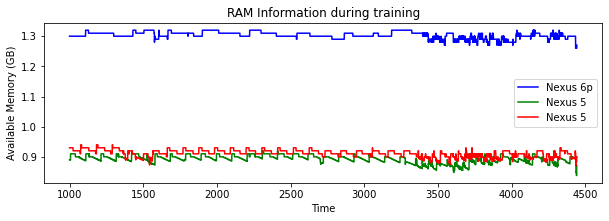
\includegraphics[scale=0.38]{freemem}

\begin{table}[h]
    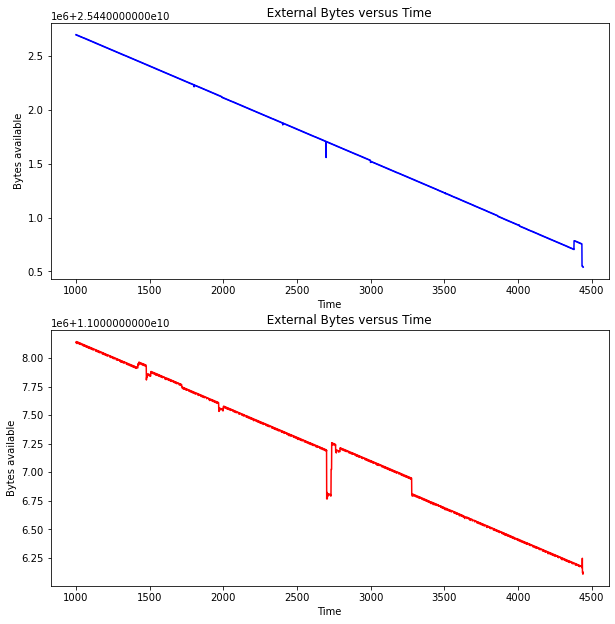
\includegraphics[scale=0.38]{extbytesvstime}
    \caption{External Bytes Available: As shown in Figure 1, since we are logging data every second, this is why the external storage bytes are constantly decreasing.}
\end{table}

\begin{table}[H]
    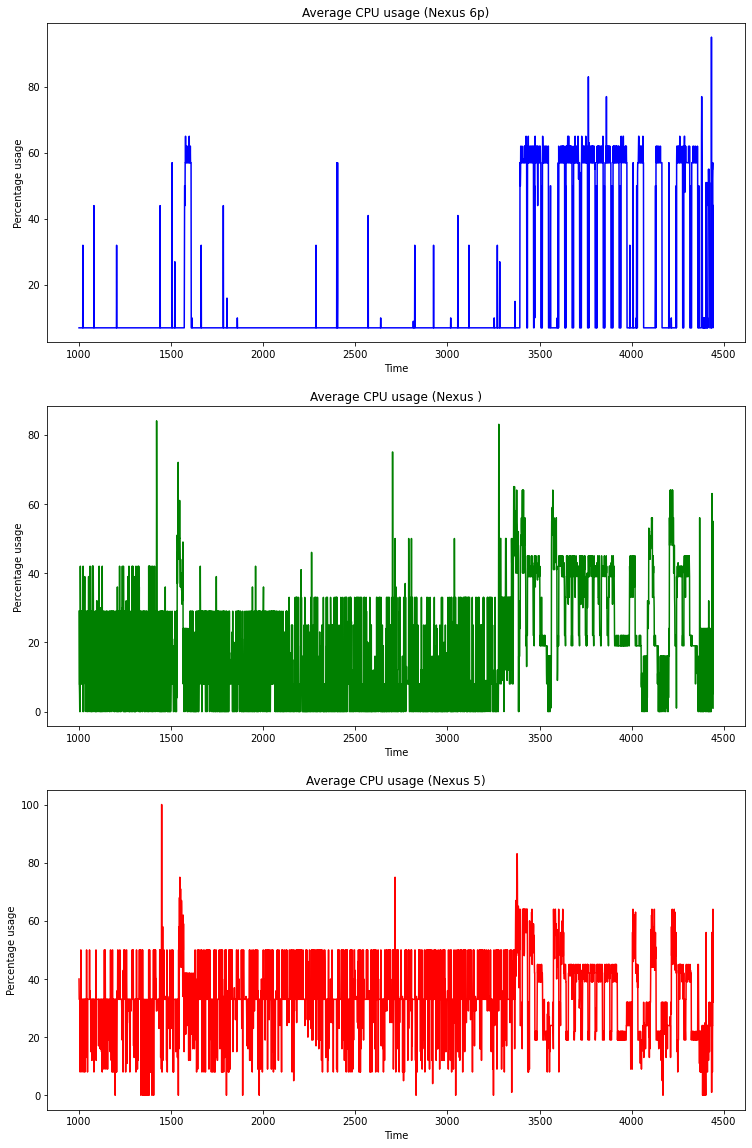
\includegraphics[scale=0.30]{cpuprof}
    \caption{CPU Profile: In the first round, training completes for each device for the set number of epochs. However, due to a systematic error, the client thread blocks and the server waits for the client parameters so no CPU is utilized for the FL task. When one of the devices was switched to the foreground, the blockage is removed and the task resumes. This is a bug in our system which we are working on fixing.}
\end{table}